\chapter{Geheimschriften und einfache Kryptosysteme}\label{ch:Geheimschriften_Kryptosysteme}

\lstset{style=Python}

\section{Einführung}\label{sec:intro}

Alice möchte Bob eine vertrauliche Nachricht (z.\,B. Bankdaten, gesundheitliche Befunde) über das Internet zukommen lassen. Nun ist das Internet ein sehr grosses physisches Netzwerk, das sich über die ganze Welt erstreckt. 
Es besteht aus unzähligen Kabeln, Routern, Servern, etc., die von verschiedenen Organisationen und Staaten betrieben werden. Wenn Alice eine Nachricht an Bob sendet, wird diese Nachricht über dieses Netzwerk transportiert und durchläuft dabei viele verschiedene Geräte und Verbindungsstrecken. 
Es ist für Alice und Bob, praktisch gesprochen, unmöglich auszuschliessen, dass jemand die Nachricht mitlesen / mithören könnte, während sie über das Internet transportiert wird.
\par

Die \emph{Kryptologie} befasst sich (unter anderem) mit der Frage, wie Alice ihre ursprüngliche Nachricht (\emph{Klartext}) vor der Übertragung so verändern kann, dass es nur für den vorgesehenen Empfänger Bob, jedoch nicht für einen unbefugten Angreifer, möglich ist, aus der veränderten Nachricht den Klartext zu rekonstruieren. Der Angreifer würde im Idealfall also lediglich einen unverständlichen \enquote{Wortsalat} mitlesen, der für ihn unverständlich ist.

\section{Geheimschriften}\label{sec:geheimschriften}
Sicherlich haben Sie als Kind schon einmal eine Geheimschrift erfunden, um geheime Nachrichten mit Ihren Freunden auszutauschen.

\begin{myexample}[Geheimschrift der Freimaurer]
Recht bekannt ist das \emph{Freimaurer-Alphabet}. Bei dieser Geheimschrift werden die lateinischen Grossbuchstaben des Klartexts durch neue Symbole ersetzt. 
Die Sicherheit dieses Verfahrens beruht allein darauf, dass die Regeln der Übersetzung geheim gehalten werden (\emph{Security through Obscurity}). 
In \cref{fig:Freimaurer} sehen Sie, wie die Geheimschrift der Freimaurer aufgebaut ist und wie die Symbole den Buchstaben zugeordnet werden.
\par
Dem Buchstaben \texttt{A} im Klartext wird zum Beispiel das Symbol {\pigpenfont A} zugeordnet, dem Buchstaben \texttt{B} das Symbol {\pigpenfont B}, dem Buchstaben \texttt{C} das Symbol {\pigpenfont C}, und so weiter. So wird zum Beispiel aus dem Klartext \texttt{HALLO} der Geheimtext {\pigpenfont HALLO}.

\begin{figure}[H]
    \centering
    \begin{subfigure}[b]{0.45\textwidth}
        \centering
		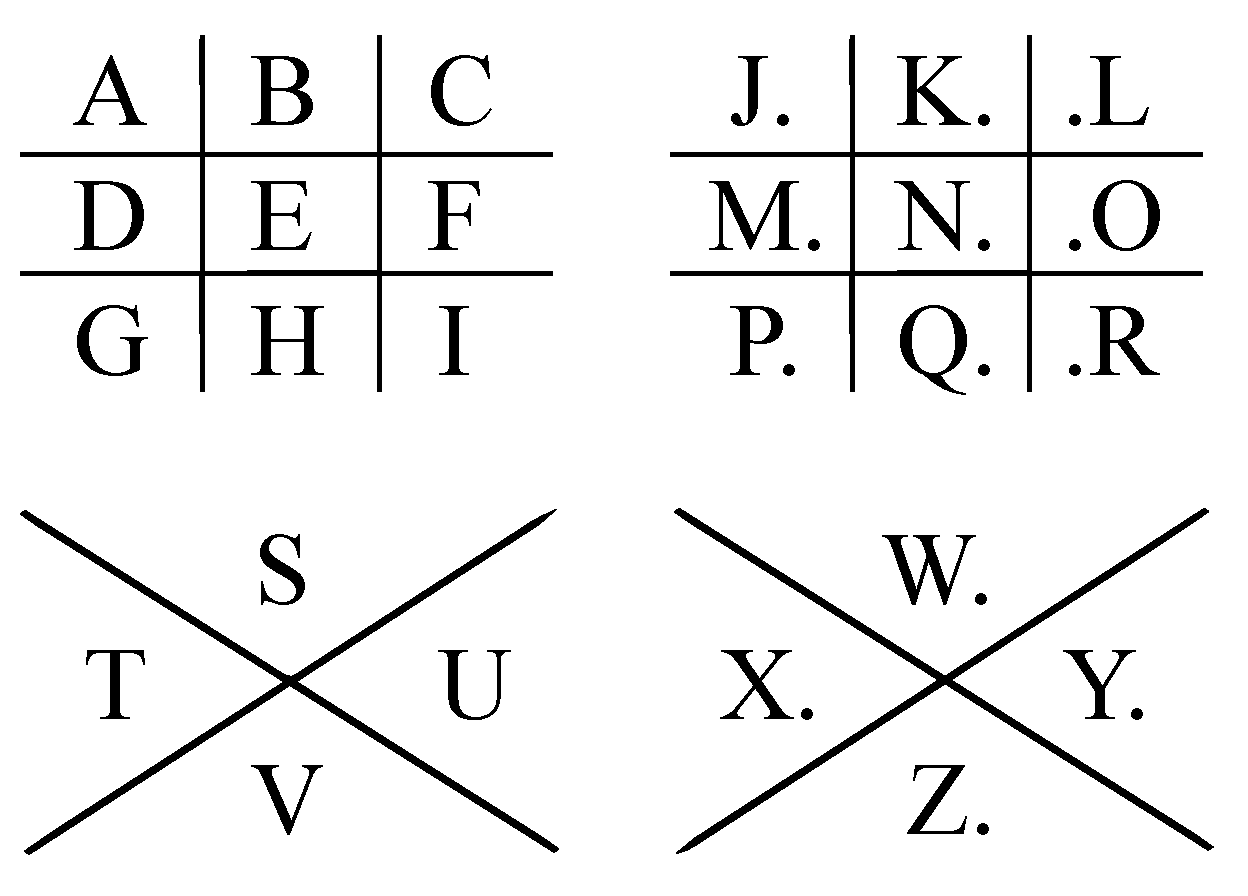
\includegraphics[width=\linewidth]{Grundlagen_Info/03_Kryptologie/Figures/Freimaurer-Alphabet.pdf} 
        \caption{Die Geheimschrift der Freimaurer.}
    \end{subfigure}
    \hfill
    \begin{subfigure}[b]{0.45\textwidth}
        \centering
        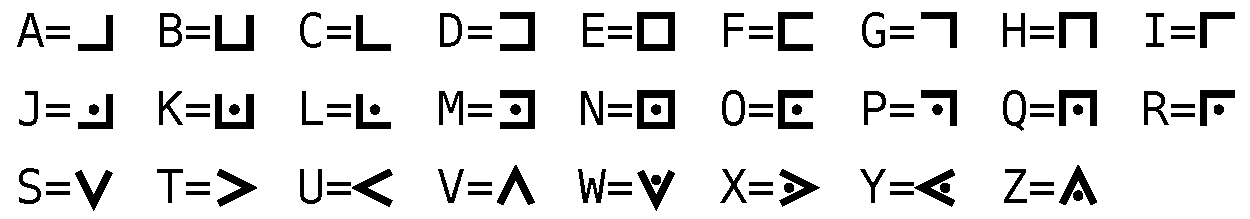
\includegraphics[width=\linewidth]{Grundlagen_Info/03_Kryptologie/Figures/Freimaurer-Buchstaben.pdf}
        \caption{Zuordnung der Symbole.}
    \end{subfigure}
    \caption[Freimaurer]{Freimaurer-Geheimschrift: Beispiel für ein Verfahren, dessen Sicherheit von der Geheimhaltung des Systems abhängt. \\ {\small Quelle: \href{https://de.wikipedia.org/wiki/Freimaurer-Alphabet}{Wikimedia Commons}}}
    \label{fig:Freimaurer}
\end{figure}
\end{myexample}

Das allgemeine Schema der Verwendung einer Geheimschrift ist in \cref{fig:schemaGeheimschrift} dargestellt. Alice (Sender) \emph{chiffriert} den Klartext, um den Geheimtext zu erhalten, und übermittelt diesen über einen unsicheren Kanal (z.\,B. Internet, Telefonie) an Bob (Empfänger). 
Bob \emph{dechiffriert} den Geheimtext, um wieder den Klartext zu erhalten. Ein Angreifer (Eve) könnte versuchen, den Geheimtext abzufangen und zu dechiffrieren, um den Klartext zu erfahren.

\begin{figure}[H]
    \centering
    \begin{tikzpicture}[mylabel/.style={text width=20mm, align=center},scale=0.8, every node/.style={scale=0.8}]
    \node[alice, minimum width=1.5cm, 
        label={[mylabel, anchor=west]north east:{}}, 
        label={[mylabel, anchor=east]north west:{\textcolor{Blue}{Klartext} $\big\downarrow\text{\tiny (Chiffrierung)}$\\
        \textcolor{Red}{Geheimtext}}}] (alice) {Alice (Sender)};
    \node[bob, minimum width=1.5cm, right=5cm of alice, mirrored,
        label={[mylabel, anchor=east]north west:{}}, 
        label={[mylabel, anchor=west]north east:{\textcolor{Red}{Geheimtext} $\big\downarrow\text{\tiny (Dechiffrierung)}$\\
        \textcolor{Blue}{Klartext}}}] (bob) {Bob (Empfänger)};
    
    \draw[->, thick, black] ([yshift=0mm]alice.east) coordinate(aux-a)-- coordinate[near start] (aux) node[above, text width=3cm, align=center]{Übermittlung über unsicheren Kanal e.g. Internet, Telefonie \\
    \textcolor{Red}{Geheimtext}} (aux-a-|bob.west);

    \node[devil, minimum width=1.5cm, below right=13mm and 1.6cm of alice] (eve) {Eve (Gegner / Abhörer)};
    \draw[<-, gray] (eve)--(aux) node[midway,right]{abhören};
    \end{tikzpicture}
    \caption{Dieses Schema zeigt die Kommunikation zwischen Alice (Sender) und Bob (Empfänger) unter Verwendung einer Geheimschrift. Der Name \emph{Eve} ist eine clevere Abkürzung für \emph{eavesdropper}, was auf Deutsch so viel wie \emph{Abhörer} bedeutet.}
    \label{fig:schemaGeheimschrift}
\end{figure}

\begin{mydefinition}[Geheimschrift]\label{mydefinition:geheimschrift}
Eine \textbf{Geheimschrift} realisiert eine Transformation (\emph{Chiffrierung}) von einem Klartext in einen Geheimtext. 
Die Umkehrung dieser Transformation (\emph{Dechiffrierung}) ermöglicht es, den Klartext aus dem Geheimtext (typischerweise eindeutig) zu rekonstruieren:
\begin{align*}
	&\text{Chiffrierung}(\text{Klartext}) = \text{Geheimtext} \\
	&\text{Dechiffrierung}(\text{Geheimtext}) = \text{Klartext}.
\end{align*}
Beispielsweise:
\begin{align*}
    &\text{Freimaurer\_Chiffrierung}(\texttt{HALLO}) = \text{\pigpenfont HALLO} \\
    &\text{Freimaurer\_Dechiffrierung}(\text{\pigpenfont HALLO}) = \texttt{HALLO}.
\end{align*}
\end{mydefinition}


\section{Von Geheimschriften zu Kryptosystemen}
Geheimschriften haben eine lange Geschichte und wurden in verschiedenen Kulturen und Epochen verwendet, um geheime Nachrichten zu übermitteln. Sie sind ein wichtiger Bestandteil der Kryptologie, da sie die Grundlage für die Entwicklung der modernen Kryptoverfahren bilden. 
Die Verwendung von Geheimschriften hat aber einen entscheidenden Nachteil: Wenn die Regeln der Geheimschrift bekannt werden, kann jeder, der den Geheimtext abfängt, diesen dechiffrieren und den Klartext lesen. Daher sind Geheimschriften allein nicht ausreichend, um die Vertraulichkeit von Nachrichten zu gewährleisten, insbesondere in einer Welt, in der Informationen leicht zugänglich und verbreitet werden können.

\begin{myremark}[\emph{Security through Obscurity}]
\emph{Security through Obscurity} (Sicherheit durch Verschleierung) bezeichnet die Praxis, die Sicherheit eines Systems dadurch zu gewährleisten, dass die Funktionsweise des Systems geheim gehalten wird. 
Die Praxis der \emph{Security through Obscurity} wird als unsicher angesehen, da sie auf der Annahme beruht, dass Angreifer nicht in der Lage sein werden, die Funktionsweise des Systems zu verstehen oder zu entdecken.
\end{myremark}

\begin{myidea}[Kryptosystem]
Wir wollen von Geheimschriften zu sogenannten \textbf{Kryptosystemen} übergehen, die so konstruiert sind, dass sie auch dann sicher sind, wenn die grundlegende Funktionsweise des Systems öffentlich bekannt ist. 
\par
Ein solches System kennen Sie bereits aus dem Alltag: Wir wissen alle, wie ein Türschloss grundsätzlich mit einem Schlüssel zu öffnen ist, aber dennoch können wir unsere Türen sicher verschliessen, da die Sicherheit nicht von der Geheimhaltung des Mechanismus abhängt, sondern von der Geheimhaltung (sicheren Aufbewahrung) des Schlüssels.
\end{myidea}

Wir werden im Folgenden einige einfache Kryptosysteme kennenlernen, um zu verstehen, was ein sicheres Kryptosystem auszeichnet.

\section{Beispiele einfacher Kryptosysteme}

\subsection{Das Kryptosystem \emph{Skytale}}
Das bereits von den Griechen für militärische Zwecke verwendete Kryptosystem \emph{Skytale} basiert auf der \textbf{Transposition}: Dabei bleiben die Buchstaben des Klartexts im Kryptotext zwar erhalten, ändern aber nach folgendem Algorithmus ihre Positionen:
\begin{itemize}
	\item Schreibe den Klartext zeilenweise in eine Tabelle (Matrix) von links nach rechts.
	\item Allfällige leere Felder in der letzten Zeile der Tabelle werden mit beliebigen (am besten zufällig gewählten) Buchstaben gefüllt.
	\item Den Kryptotext erhalten wir, indem wir die Buchstaben Spalte für Spalte von links nach rechts und von oben nach unten lesen.
\end{itemize}

Die Skytale wird mit einem Stab und einem Band umgesetzt (\cref{fig:skytale-band}). Die Anzahl der Zeichen pro Windung entspricht dabei der Zeilenanzahl der Tabelle und bildet somit den Schlüssel.

\begin{figure}[H]
	\centering
	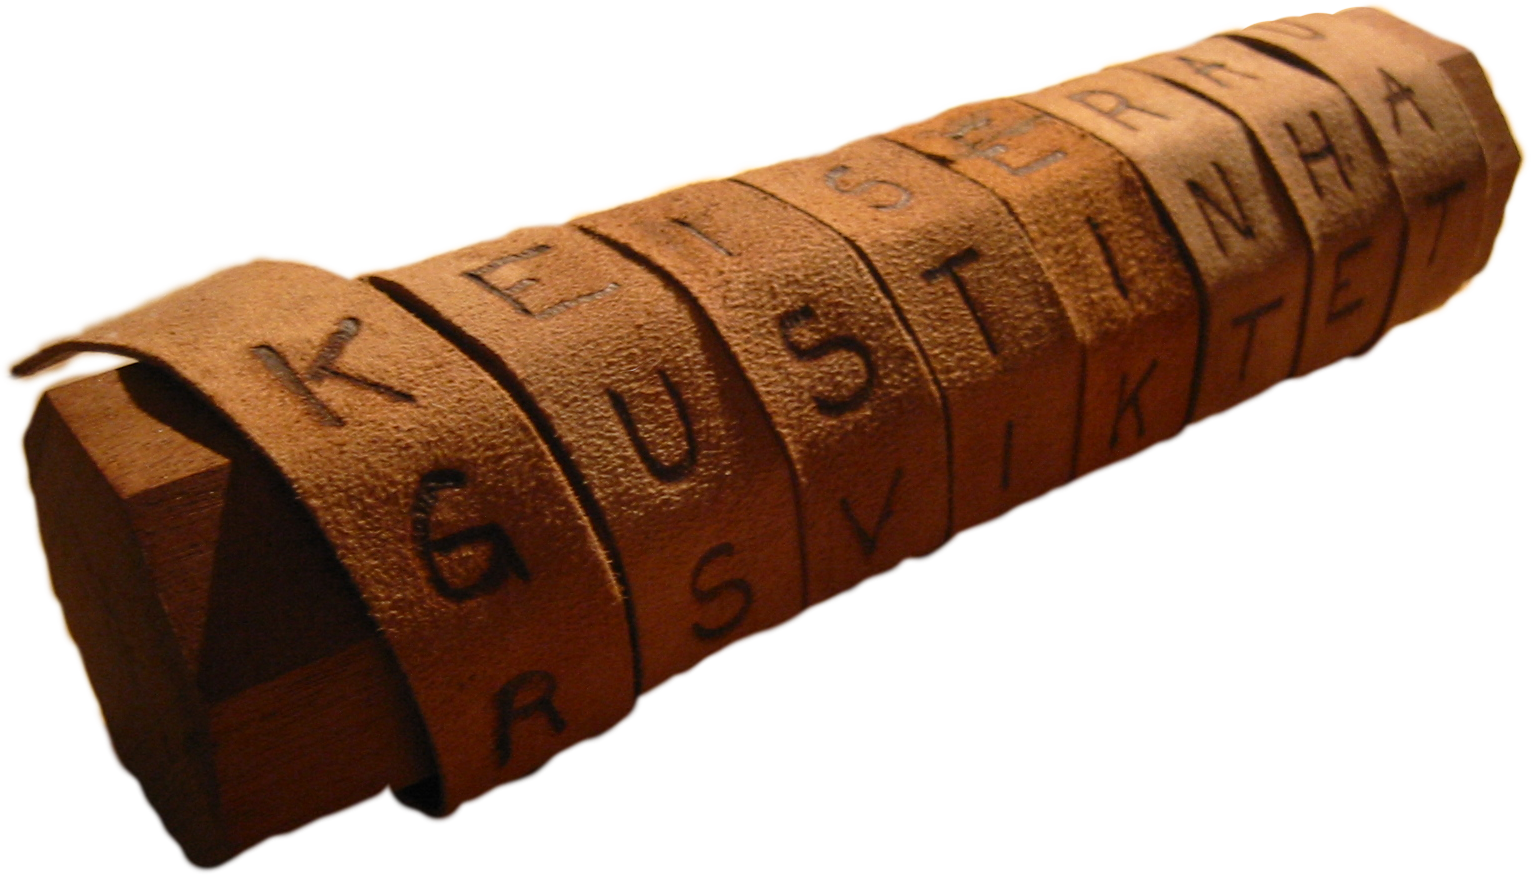
\includegraphics[width=0.5\linewidth]{Grundlagen_Info/03_Kryptologie/Figures/SkytaleWiki}
	\caption[Skytale]{Praktische Umsetzung der Skytale-Verschlüsselung mit einem Stab und einem Band. 
	Die Anzahl Zeichen, die auf eine Windung des Bandes um den Stab passen, entspricht der Anzahl Zeilen in der Tabelle, also dem Schlüssel des Kryptosystems \emph{Skytale}. \\ {\small Quelle: \href{https://commons.wikimedia.org/wiki/File:Skytale.png}{Wikimedia Commons}}}
	\label{fig:skytale-band}
\end{figure}

\begin{myexercise}
	Der Kryptotext
	\begin{center}
		\texttt{WNGIAEIEMATSMKRTTEAGIEINANINTUGNDOJEEENL}
	\end{center}
	wurde mit einer Tabelle mit 5 Zeilen und 8 Spalten erzeugt. Wie lautet der Klartext? Tipp: Nehmen Sie Ihr bevorzugtes Tabellenkalkulationsprogramm zuhilfe.
	\begin{myanswer}

		Wir beginnen mit einer leeren $5\times 8$ Tabelle und schreiben den gegebenen Kryptotext spaltenweise von links nach rechts und von oben nach unten in die Tabelle ein:
		\begin{table}[H]
			\centering
			\begin{tabular}{*{8}{C|}} % 8 Spalten vom Typ C (mit Linien)
				W & E & T & T & I & N & G & E \\ \hline
				N & I & S & T & E & I & N & E \\ \hline
				G & E & M & E & I & N & D & E \\ \hline
				I & M & K & A & N & T & O & N \\ \hline
				A & A & R & G & A & U & \textcolor{Red}{J} & \textcolor{Red}{L}
			\end{tabular}
		\end{table}
		Der Klartext
		\begin{center}
			\texttt{Wettingen ist eine Gemeinde im Kanton Aargau}
		\end{center}
		lässt sich nun einfach ablesen (Zeile für Zeile von links nach rechts).
	\end{myanswer}
\end{myexercise}

\begin{myexercise}
	Der folgende Kryptotext der Länge 75 wurde mit Skytale verschlüsselt:
	\begin{center}
		\texttt{ETIFIITNUTNFGENKURRELEODIERSILIMSEANIE}\\
		\texttt{MRECREMRHSNSSAPSTCBRCRHEUHORRNHNIEGEG}
	\end{center}
	Dabei konnten mit dem Klartext \textbf{alle Zeilen der Tabelle vollständig aufgefüllt} werden.
	\begin{enumerate}
		\item Wie viele verschiedene Schlüssel (Anzahl Zeilen) sind in dieser Situation möglich?
		\item Welcher Schlüssel wurde hier verwendet? Tipp: Sie können \href{https://cryptbreaker.marcwidmer.xyz/solve}{diesen Link} mit \emph{Analysewerkzeug} $\rightarrow$ \emph{Tabelle} dazu verwenden.
		\item Wie lautet der Klartext?
	\end{enumerate}

	\begin{myanswer}
	\begin{table}[H]
		\centering
		% *{15}{C|} bedeutet: 15-mal den Typ 'C' mit Trennlinie
		\begin{tabular}{*{15}{C|}} 
			E & I & N & K & L & E & I & N & E & R & S & C & H & R & I \\ \hline
			T & T & F & U & E & R & M & I & C & H & A & B & E & R & E \\ \hline
			I & N & G & R & O & S & S & E & R & S & P & R & U & N & G \\ \hline
			F & U & E & R & D & I & E & M & E & N & S & C & H & H & E \\ \hline
			I & T & N & E & I & L & A & R & M & S & T & R & O & N & G
		\end{tabular}
	\end{table}
		\begin{enumerate}
			\item Wir müssen $75$ Buchstaben auf ein Rechteck verteilen. Damit kommen alle Teiler von $75$, also 1, 3, 5 und 75, als mögliche Schlüssel in Frage. 
			\item Durch Ausprobieren finden wir, dass einzig der Schlüssel 5 zu einem sinnvollen Klartext führt.
			\item Der Klartext lautet:
			      \begin{center}
				      {\small
					      \texttt{EIN KLEINER SCHRITT FUER MICH ABER EIN GROSSER}\\
					      \texttt{SPRUNG FUER DIE MENSCHHEIT NEIL ARMSTRONG}}
			      \end{center}
		\end{enumerate}
	\end{myanswer}
\end{myexercise}

\begin{myexercise}
	Sie möchten einen Klartext der Länge 87 mit Hilfe einer Tabelle mit 10 Zeilen verschlüsseln. Wie viele Spalten benötigt diese Tabelle?
	\begin{myanswer}
		Die Tabelle benötigt 9 Spalten. Allgemein lässt sich die Anzahl benötigter Spalten berechnen durch
		\begin{align*}
			\ceil{\frac{\text{Länge des Textes}}{\text{Anzahl Zeilen}}}, \qquad \text{wobei } \ceil{...} \text{ die Aufrundungsfunktion ist.}
		\end{align*}
	\end{myanswer}
\end{myexercise}

\begin{myexercise}\label{ex:zweiertausch}
	Wie die Skytale, beruht auch die folgende Verschlüsselungsmethode auf der Transposition von Buchstaben. 
	Finden Sie zu den folgenden Kryptotexten die Klartexte (unverschlüsselte Nachrichten):
	\begin{center}
		\small
		\begin{enumerate}
			\item \texttt{RKPYOTOLIGEEMREOLGCITHEGEHMIINSSE}
			\item \texttt{HCSFIRILTAHCZFUEBUHAWNERDNUKUZMMOINUEIZNER}
		\end{enumerate}
		\normalsize
	\end{center}

	\begin{myanswer}
		Ursprünglicher Text:
		\begin{center}
			\small
			\begin{enumerate}
				\item \texttt{KRYPTOLOGIE ERMOEGLICHT GEHEIMNISSE}
				\item \texttt{SCHRIFTLICH AUFZUBEWAHREN UND ZU KOMMUNIZIEREN}
			\end{enumerate}
			\normalsize
		\end{center}
		Der Kryptotext entsteht durch Austauschen der Positionen der Buchstaben, wie gezeigt in \cref{fig:transposition-cipher}.
		\begin{figure}[H]
            \centering
            \begin{subfigure}[b]{0.48\textwidth}
                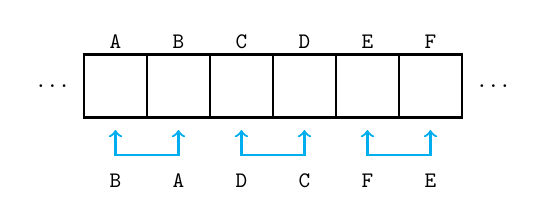
\begin{tikzpicture}[scale=0.8, every node/.style={scale=0.8, font=\ttfamily}]
                    % Parameters
                    \def\boxwidth{1} % Width of each box
                    \def\numboxes{6} % Total number of boxes
                    \pgfmathtruncatemacro{\lastindex}{\numboxes-2} 
                    \pgfmathtruncatemacro{\lastindexLet}{\numboxes-1} 

                    % Draw the rectangle
                    \draw[thick] (0, 0) rectangle (\numboxes*\boxwidth, 1);
                    \foreach \i in {1,...,\numboxes} {
                            \draw[thick] (\i*\boxwidth, 0) -- (\i*\boxwidth, 1);
                        }

                    % Add ellipses
                    \node at (-0.5, 0.5) {\dots};
                    \node at (\numboxes*\boxwidth+0.5, 0.5) {\dots};

                    % Add arrows for swapping
                    \foreach \i in {0,2,...,\lastindex} {
                            \pgfmathsetmacro{\xstart}{\i*\boxwidth + 0.5*\boxwidth}
                            \pgfmathsetmacro{\xend}{\xstart + \boxwidth}
                            \draw[thick, cyan, <->] (\xstart, -0.2) -- (\xstart, -0.6) -- (\xend, -0.6) -- (\xend, -0.2);
                        }

                    % Add letters above
                    \foreach \i in {0,...,\lastindexLet} {
                            \pgfmathsetmacro{\xpos}{\i*\boxwidth + 0.5*\boxwidth}
                            \pgfmathtruncatemacro{\letter}{65+\i} 
                            \node at (\xpos, 1.2) {\char\letter};
                        }

                    % Add swapped letters below
                    \foreach \i in {0,...,\lastindexLet} {
                            \pgfmathsetmacro{\xpos}{\i*\boxwidth + 0.5*\boxwidth}
                            \ifodd\i
                                \pgfmathtruncatemacro{\swapletter}{65+\i-1} 
                            \else
                                \pgfmathtruncatemacro{\swapletter}{65+\i+1} 
                            \fi
                            \node at (\xpos, -1) {\char\swapletter};
                        }
                \end{tikzpicture}
                \caption{\enquote{Zweiertausch}}
            \end{subfigure}
            \hspace{0.1cm}
            \begin{subfigure}[b]{0.48\textwidth}
                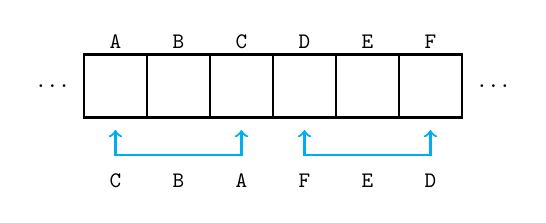
\begin{tikzpicture}[scale=0.8, every node/.style={scale=0.8, font=\ttfamily}]
                    % Parameters
                    \def\boxwidth{1} 
                    \def\numboxes{6} 
                    \pgfmathtruncatemacro{\lastindex}{\numboxes-3} 
                    \pgfmathtruncatemacro{\lastindexLet}{\numboxes-1} 

                    % Draw the rectangle
                    \draw[thick] (0, 0) rectangle (\numboxes*\boxwidth, 1);
                    \foreach \i in {1,...,\numboxes} {
                            \draw[thick] (\i*\boxwidth, 0) -- (\i*\boxwidth, 1);
                        }

                    % Add ellipses
                    \node at (-0.5, 0.5) {\dots};
                    \node at (\numboxes*\boxwidth+0.5, 0.5) {\dots};

                    % Add arrows for swapping
                    \foreach \i in {0,3,...,\lastindex} {
                            \pgfmathsetmacro{\xstart}{\i*\boxwidth + 0.5*\boxwidth}
                            \pgfmathsetmacro{\xend}{\xstart + \boxwidth*2}
                            \draw[thick, cyan, <->] (\xstart, -0.2) -- (\xstart, -0.6) -- (\xend, -0.6) -- (\xend, -0.2);
                        }

                    % Add letters above
                    \foreach \i in {0,...,\lastindexLet} {
                            \pgfmathsetmacro{\xpos}{\i*\boxwidth + 0.5*\boxwidth}
                            \pgfmathtruncatemacro{\letter}{65+\i} 
                            \node at (\xpos, 1.2) {\char\letter};
                        }

                    % Add swapped letters below
                    \foreach \i in {0,3,...,\lastindex} {
                            \pgfmathtruncatemacro{\swapletter}{65+\i+2} 
                            \pgfmathsetmacro{\xpos}{\i*\boxwidth + 0.5*\boxwidth}
                            \node at (\xpos, -1) {\char\swapletter};
                        }

                    \foreach \i in {2,5,...,\numboxes} {
                            \pgfmathtruncatemacro{\swapletter}{65+\i-2} 
                            \pgfmathsetmacro{\xpos}{\i*\boxwidth + 0.5*\boxwidth}
                            \node at (\xpos, -1) {\char\swapletter};
                        }

                    \foreach \i in {1,4,...,\lastindexLet} {
                            \pgfmathtruncatemacro{\swapletter}{65+\i} 
                            \pgfmathsetmacro{\xpos}{\i*\boxwidth + 0.5*\boxwidth}
                            \node at (\xpos, -1) {\char\swapletter};
                        }
                \end{tikzpicture}
                \caption{\enquote{Dreiertausch}}
            \end{subfigure}
            \caption{\enquote{Zweiertausch} und \enquote{Dreiertausch}}
            \label{fig:transposition-cipher}
        \end{figure}
		Beachten Sie, dass die Buchstaben des Klartexts im Kryptotext erhalten bleiben, aber ihre Reihenfolge geändert wird. Die Schlüssel für diese Kryptosystem sind die Anweisungen, wie die Buchstaben vertauscht werden, z.\,B. \enquote{Zweiertausch} oder \enquote{Dreiertausch}.
	\end{myanswer}
\end{myexercise}


\subsection{Das Kryptosystem \emph{Caesar}}
\label{subsec:caesar}
Eines der bekanntesten Kryptosysteme der Antike ist die Caesar-Verschlüsselung, die von Julius Caesar verwendet wurde. 
Dabei wird jeder Buchstabe des Klartexts um eine feste Anzahl von Positionen im Alphabet verschoben. 
Die Anzahl der Positionen, um die verschoben wird, bildet den Schlüssel des Kryptosystems.

\begin{myremark}[Buchstaben als Zahlen]\label{myremark:buchstaben_als_zahlen}
Häufig wird die Verschiebung nicht direkt als Zahl angegeben, sondern als Buchstabe, der die Anzahl der Positionen angibt. So steht beispielsweise der Schlüssel \texttt{A} für eine Verschiebung um 0 Positionen (keine Verschiebung), \texttt{B} für eine Verschiebung um 1 Position, \texttt{C} für eine Verschiebung um 2 Positionen, \texttt{D} für eine Verschiebung um 3 Positionen und so weiter:
\begin{center}
	\texttt{A} $\leftrightarrow$ 0 Positionen, \texttt{B} $\leftrightarrow$ 1 Position, \texttt{C} $\leftrightarrow$ 2 Positionen, \dots , \texttt{Z} $\leftrightarrow$ 25 Positionen.
\end{center}
\end{myremark}

\begin{mydefinition}[Ordnung eines Buchstabens]\label{mydefinition:ordnung_buchstabe}
Die \textbf{Ordnung} eines Buchstabens ist die Anzahl der Positionen, die dieser Buchstabe im Alphabet von \texttt{A} entfernt ist. Wir definieren
\begin{center}
	$\text{Ord}(\texttt{A}) = 0$, $\text{Ord}(\texttt{B}) = 1$, $\text{Ord}(\texttt{C}) = 2$, \dots, $\text{Ord}(\texttt{Z}) = 25$.
\end{center}
\end{mydefinition}

\begin{myexample}[Caesar mit Schlüssel \texttt{D}]
Mit dem Schlüssel \texttt{D} (3 Positionen, da $\text{Ord}(\texttt{D}) = 3$)  wird aus dem Klartext \texttt{HALLO} der Kryptotext \texttt{KDOOR}:
\begin{figure}[H]
	\centering
	\caesar[3]
	\label{fig:caesar_3}
\end{figure}
Dabei haben wir die innere Scheibe um 3 Positionen im Uhrzeigersinn gedreht, um die Verschlüsselung durchzuführen (\enquote{lesen von innen nach aussen}). Zur Entschlüsselung
\begin{itemize}
	\item lesen wir die Drehscheiben, genau so wie sie in \cref{fig:caesar_3} angeordnet sind, von \enquote{aussen nach innen}
	\item oder drehen die innere Scheibe um 3 Positionen gegen den Uhrzeigersinn zurück in die Ausgangsposition (\texttt{A} $\leftrightarrow$ \texttt{A}) und dann nochmals um 3 Positionen gegen den Uhrzeigersinn (dies können wir um eine Verschiebung um $-3$ Positionen anschauen). 
	Mit diesem Vorgehen können wir die Drehscheiben wieder von \enquote{innen nach aussen} lesen, um den Klartext zu erhalten.
\end{itemize}
\url{https://www.101computing.net/cipher-wheel.html}{Hier} finden Sie ein interaktives Werkzeug, um die Caesar-Verschlüsselung und -Entschlüsselung durchzuführen. 
\end{myexample}

\begin{myexample}
Folgender Text wurde mit dem Schlüssel \texttt{G} (6 Positionen) verschlüsselt:

\begin{verbatim}
Klartext: JEMANDMUSSTEJOSEFKVERLEUMDETHA...
Schlüssel: GGGGGGGGGGGGGGGGGGGGGGGGGGGGGG...
Kryptotext: PKSGTJSAYYZKPUYKLQBKXRKASJKZNG...
\end{verbatim}
\end{myexample}

\begin{myexercise}\label{myexercise:vorbetrachung_haeufigkeitsanalyse}
	Der Kryptotext
	\begin{center}
		\texttt{X G T Y G P F G U E J N W G U U G N B Y G K}
	\end{center}
	wurde mit Caesar verschlüsselt, der Schlüssel ist aber unbekannt.
	Entschlüsseln Sie den Kryptotext, ohne alle Schlüssel auszuprobieren, wenn Sie wissen, dass der häufigste Buchstabe im Klartext \texttt{E} ist.
	\begin{myanswer}
		Der häufigste Buchstabe im Kryptotext ist \texttt{G}. Wir vermuten also, dass die \texttt{G}'s im gegebenen Kryptotext aus den \texttt{E}'s im Klartext entstanden. Dies entspricht einer Verschlüsselung mit dem Schlüssel 2 bzw. \texttt{C}. Wir können den Text mithilfe der Verschiebung \texttt{G} $\rightarrow$ \texttt{E} entschlüsseln:
		\begin{center}
			\caesar[2]\\
			\texttt{V E R W E N D E D E N S C H L U E S S E L Z W E I}
		\end{center}
	Dazu lesen wir von \enquote{aussen nach innen} (Entschlüsselung).
	\end{myanswer}
\end{myexercise}


\section{Allgemeine Betrachtungen zu Kryptosystemen}
\subsection{Definition eines Kryptosystems}
Ein Kryptosystem besteht aus einem Verschlüsselungsalgorithmus, einem Entschlüsselungsalgorithmus und einem Schlüssel. 
Der Verschlüsselungsalgorithmus nimmt den Klartext und den Schlüssel als Eingabe und erzeugt den Kryptotext. Der Entschlüsselungsalgorithmus nimmt den Kryptotext und den Schlüssel als Eingabe und rekonstruiert den Klartext. 
Die Sicherheit eines Kryptosystems sollte nicht davon abhängen, dass die Funktionsweise des Systems geheim gehalten wird, sondern allein von der Geheimhaltung des Schlüssels.
\par
Das Schema in \cref{fig:schemaKryptosystem} zeigt die Kommunikation zwischen Alice (Sender) und Bob (Empfänger) unter Verwendung eines Kryptosystems. Alice verschlüsselt den Klartext mit dem Schlüssel, um den Kryptotext zu erhalten, und übermittelt diesen über einen unsicheren Kanal (z.\,B. Internet, Telefonie) an Bob. Bob benötigt den Schlüssel, um den Kryptotext zu entschlüsseln und den Klartext zu erhalten. Ein Angreifer (Eve) könnte versuchen, den Kryptotext abzufangen und zu entschlüsseln, um den Klartext zu erfahren.
\begin{figure}[H]
	\centering
	\begin{tikzpicture}[mylabel/.style={text width=20mm, align=center},scale=0.8, every node/.style={scale=0.8}]
		\node[alice, minimum width=1.5cm,
		label={[mylabel, anchor=west]north east:{}},
		label={[mylabel, anchor=east]north west:{\textcolor{Blue}{(Klartext, Schlüssel)} $\big\downarrow\text{\tiny (Verschlüsselung)}$\\
		\textcolor{Red}{\mbox{Kryptotext}}}}] (alice) {Alice (Sender)};
		\node[bob, minimum width=1.5cm, right=5cm of alice, mirrored,
		label={[mylabel, anchor=east]north west:{}},
		label={[mylabel, anchor=west]north east:{\textcolor{Red}{(\mbox{Kryptotext}, Schlüssel)} $\big\downarrow\text{\tiny (Entschlüsselung)}$\\
		\textcolor{Blue}{Klartext}}}] (bob) {Bob (Empfänger)};

		\draw[->, thick, black] ([yshift=0mm]alice.east) coordinate(aux-a)-- coordinate[near start] (aux) node[above, text width=3cm, align=center]{Übermittlung über unsicheren Kanal e.g. Internet, Telefonie \\
				\textcolor{Red}{Kryptotext}} (aux-a-|bob.west);

		\node[devil, minimum width=1.5cm, below right=13mm and 1.6cm of alice] (eve) {Eve (Gegner / Abhörer)};
		\draw[<-, gray] (eve)--(aux) node[midway,right]{abhören};
	\end{tikzpicture}
	\caption{Kommunikation zwischen Alice (Sender) und Bob (Empfänger) unter Verwendung eines Kryptosystems. Bob benötigt den Schlüssel, um den Kryptotext zu entschlüsseln.}
	\label{fig:schemaKryptosystem}
\end{figure}

\begin{mydefinition}[Kryptosystem]\label{mydefinition:kryptosystem}
	Ein \textbf{Kryptosystem} realisiert eine Transformation (\emph{Verschlüsselung}) von einem Klartext in einen Kryptotext, die von einem Schlüssel abhängt. 
	Die Menge aller möglichen Schlüssel wird \emph{Schlüsselmenge} des Kryptosystems genannt.
	Die Umkehrung dieser Transformation (\emph{Entschlüsselung}) ermöglicht es, den Klartext aus dem Kryptotext zu rekonstruieren, wenn man den Schlüssel kennt:
	\begin{align*}
		&\text{Verschlüsselung}(\text{Klartext}, \text{Schlüssel}) = \text{Kryptotext} \\
		&\text{Entschlüsselung}(\text{Kryptotext}, \text{Schlüssel}) = \text{Klartext}.
	\end{align*}
	Beispielsweise (mit Caesar):
	\begin{align*}
		&\text{Verschlüsselung}(\texttt{HALLO}, 3) = \texttt{KDOOR} \\
		&\text{Entschlüsselung}(\texttt{KDOOR}, 3) = \texttt{HALLO}.
	\end{align*}
	Schlüsselmenge Caesar: $\lrc{0, 1, \dots, 25}$ oder $\lrc{\texttt{A}, \texttt{B}, \dots, \texttt{Z}}$.	
\end{mydefinition}

\begin{myremark}[Geheimschrift als Spezialfall eines Kryptosystems]
	Eine Geheimschrift ist ein Spezialfall eines Kryptosystems, bei dem die Schlüsselmenge nur ein einziges Element enthält, nämlich die Anweisung, wie die Buchstaben vertauscht werden. 
	Umgekehrt, kann ein Kryptosystem als eine Sammlung von Geheimschriften betrachtet werden, wobei für jede mögliche Schlüssel eine Geheimschrift definiert ist, die die Buchstaben entsprechend der Verschlüsselungsregel vertauscht.
\end{myremark}

\subsection{Kerckhoffs'sches Prinzip}
Der niederländische Kryptologe und Linguist \emph{Auguste Kerckhoffs} stellte im Jahr 1883 die folgende Anforderung an die Sicherheit von Kryptosystemen auf, die heute als \textbf{Kerckhoffs'sches Prinzip} bekannt ist: 

\begin{myquote}\label{myquote:kerckhoffs}
	\enquote{Ein Kryptosystem sollte auch dann sicher sein, wenn alles über das System bekannt ist, ausser dem Schlüssel.} -- Auguste Kerckhoffs, \emph{La cryptographie militaire} (1883)\footnote{Originalzitat: \enquote{Il faut qu'il n'exige pas le secret, et qu'il puisse sans inconvénient tomber entre les mains de l'ennemi.}}
\end{myquote}

\begin{figure}[H]
	\centering
	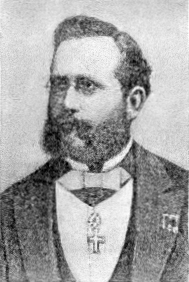
\includegraphics[width=0.3\linewidth]{Grundlagen_Info/03_Kryptologie/Figures/kerckhoffs}
	\caption{Auguste Kerckhoffs (1835--1903)}
	\label{fig:kerckhoffs}
\end{figure}

Das Kerckhoffs'sche Prinzip besagt, dass die Sicherheit eines Kryptosystems nicht davon abhängen sollte, dass die Funktionsweise des Systems geheim gehalten wird. Stattdessen sollte die Sicherheit allein auf der Geheimhaltung des Schlüssels beruhen. Einem solchen System wird auch dann noch vertraut, wenn es öffentlich bekannt ist, da die Sicherheit nicht von der Geheimhaltung des Algorithmus abhängt, sondern von der Geheimhaltung des Schlüssels. Demgegenüber steht die Praxis der \emph{Security through Obscurity}, bei der die Sicherheit eines Systems dadurch gewährleistet wird, dass die Funktionsweise des Systems geheim gehalten wird. Diese Praxis wird als unsicher angesehen, da sie auf der Annahme beruht, dass Angreifer nicht in der Lage sein werden, die Funktionsweise des Systems zu verstehen oder zu entdecken (siehe \cref{myremark:security_through_obscurity}).

\subsection{Sicherheitsanforderungen an moderne Kryptosysteme}
Folgende Sicherheits-bezogenen Anforderungen können zusätzlich an moderne Kryptosysteme gestellt werden:
\begin{enumerate}
	\item \textbf{Vertraulichkeit}: Es soll sichergestellt sein, dass wirklich nur diejenige Person eine Nachricht lesen kann, für die diese bestimmt ist.
	\item \textbf{Integrität}: Der Empfänger soll feststellen können, ob die Nachricht nach ihrer Erzeugung verändert wurde (wir wollen ja die originale Nachricht!).
	\item \textbf{Authentizität}: Die Verfasserin einer Nachricht soll identifizierbar sein, bzw. der Empfänger soll nachprüfen können, wer die Verfasserin ist.
	\item \textbf{Verbindlichkeit}: Die Verfasserin soll nicht abstreiten können, dass sie die Verfasserin der Nachricht ist.
\end{enumerate}


% \begin{mychallenge}
% Implementieren Sie die Caesar-Verschlüsselung in Python. Einige nützliche Funktionen, die Sie für Zeichenketten verwenden können, finden SIe in:
%
%
% \begin{myanswer}
% \lstinputlisting{Grundlagen_Info/03_Kryptologie/Python package/encryption/caesar.py}
% \end{myanswer}
% \end{mychallenge}


\section{Kryptoanalyse von Caesar}
Die Caesar-Verschlüsselung ist ein einfaches Kryptosystem, das leicht zu knacken ist. Es gibt zwei Hauptmethoden, um den Schlüssel zu bestimmen und den Klartext zu rekonstruieren:
\begin{itemize}
	\item Einerseits reicht es, alle 26 (0 bis 25) möglichen Verschiebungen auszuprobieren. Ein moderner Computer hat dies in einigen Millisekunden erledigt. Natürlich muss ein Angreifer auch die Möglichkeit haben, den Klartext zu erkennen, wenn er ihn sieht, z.\,B. durch die Erkennung von sinnvollen Wortteilen (e.g. Abgleich mit einem deutschen Wörterbuch).
	\item Andererseits kann, wenn der Text genügend lang ist, anhand der Häufigkeit der verschlüsselten Buchstaben mittels einer sogenannten \emph{Häufigkeitsanalyse} in kürzester Zeit bestimmt werden, was der Schlüssel war (vielleicht erinneren Sie sich noch an \cref{myexercise:vorbetrachung_haeufigkeitsanalyse}). 
	\cref{fig:caesar-freq} zeigt die Häufigkeiten der Buchstaben eines langen, mit Caesar verschlüsselten Texts im Kryptotext.
\end{itemize}

\begin{figure}[H]
	\centering
	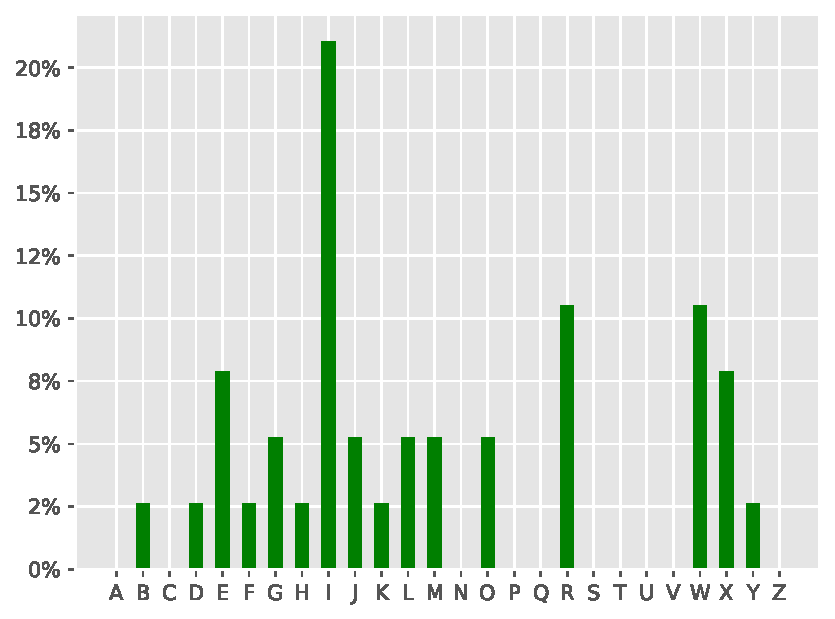
\includegraphics[width=0.7\linewidth]{Grundlagen_Info/03_Kryptologie/Figures/caesar-freq-exercise}
	\caption{Buchstabenhäufigkeit in einem nach Caesar verschlüsselten Text}
	\label{fig:caesar-freq}
\end{figure}

Die durchschnittlichen Häufigkeiten von Buchstaben, Bi- und Tri-Grammen in deutschen Texten ist in \cref{tab:alle-haeufigkeiten} angegeben.

\begin{table}[H]
	\centering
	\begin{subtable}[t]{0.3\textwidth}
		\centering
		\begin{tabular}{C|p{1.9cm}}
			\textbf{Buchstabe} & Relative Häufigkeit (\%) \\ \midrule
			E                  & 17.40                    \\ \midrule
			N                  & 9.78                     \\ \midrule
			I                  & 7.55                     \\ \midrule
			S                  & 7.27                     \\ \midrule
			R                  & 7.00                     \\ \midrule
			A                  & 6.51                     \\ \midrule
			T                  & 6.15                     \\ \midrule
			D                  & 5.08                     \\ \midrule
			H                  & 4.76                     \\ \midrule
			U                  & 4.35                     \\
		\end{tabular}
		\caption{Buchstabenhäufigkeit}
	\end{subtable}
	\hspace{0.5cm}
	\begin{subtable}[t]{0.3\textwidth}
		\centering
		\begin{tabular}{C|p{1.9cm}}
			\textbf{Bigramm} & Relative Häufigkeit (\%) \\ \midrule
			ER               & 3.94                     \\ \midrule
			EN               & 3.07                     \\ \midrule
			CH               & 2.73                     \\ \midrule
			DE               & 2.41                     \\ \midrule
			EI               & 2.29                     \\ \midrule
			ND               & 2.07                     \\ \midrule
			IE               & 1.97                     \\ \midrule
			GE               & 1.88                     \\ \midrule
			TE               & 1.88                     \\ \midrule
			IN               & 1.82                     \\
		\end{tabular}
		\caption{Bigrammhäufigkeit}
	\end{subtable}
	\hspace{0.5cm}
	\begin{subtable}[t]{0.3\textwidth}
		\centering
		\begin{tabular}{C|p{1.9cm}}
			\textbf{Trigramm} & Relative Häufigkeit (\%) \\ \midrule
			DER               & 1.44                     \\ \midrule
			SCH               & 1.21                     \\ \midrule
			ICH               & 1.08                     \\ \midrule
			DIE               & 0.98                     \\ \midrule
			UND               & 0.95                     \\ \midrule
			DEN               & 0.78                     \\ \midrule
			CHE               & 0.77                     \\ \midrule
			EIN               & 0.75                     \\ \midrule
			NDE               & 0.74                     \\ \midrule
			GEN               & 0.72                     \\
		\end{tabular}
		\caption{Trigrammhäufigkeit}
	\end{subtable}
	\caption{Relative Häufigkeiten der Buchstaben, Bigramme und Trigramme im Deutschen}
	\label{tab:alle-haeufigkeiten}
\end{table}

\begin{myexercise}\label{ex:caesar}
	Können Sie aus \cref{tab:alle-haeufigkeiten} entschlüsseln, was der Klartext ist?

	Kryptotext:

	\texttt{WMILEFIRIWKIWGLEJJXHMIWIRXIBXDYOREGOIR}

	\begin{myanswer}
		Offensichtlich ist der häufigste Buchstabe im Kryptotext \texttt{I} und der häufigste Buchstabe in deutschen Texten ist der Buchstabe \texttt{E}, wir haben hier also vermutlich eine Verschiebung von \texttt{E} zu \texttt{I}, also eine Verschiebung um 4 Stellen. Der Klartext lautet daher: \texttt{SIEHABENESGESCHAFFTDIESENTEXTZUKNACKEN}
	\end{myanswer}
\end{myexercise}

\begin{myexercise}
	Kann man immer wie in \cref{ex:caesar} vorgehen? In welchen Fällen funktioniert dieses Vorgehen eventuell nicht?
	\begin{myanswer}
		Falls der Text zu kurz ist, funktioniert die Häufigkeitsanalyse nicht immer, da der häufigste Buchstabe im Originaltext nicht immer der Buchstabe \texttt{E} ist. Dies wird beispielsweise im Klartext \texttt{WORT} illustriert, das keinen Buchstaben \texttt{E} enthält. In diesem Fall müsste man alle 26 möglichen Verschiebungen durchprobieren.
	\end{myanswer}
\end{myexercise}

\begin{mychallenge}
	Um zu verschlüsseln, liest man die Caesar-Drehscheiben von innen (Klartext) nach aussen (Kryptotext). Um zu entschlüsseln, liest man von aussen (Kryptotext) nach innen (Klartext). Gibt es Schlüssel bei Caesar, bei denen es sowohl für die Ver- wie Entschlüsselung keine Rolle spielt, in welche Richtung man die Scheiben liest?
	\begin{myanswer}
		Ja, dies tritt bei Schlüsseln 0 (\texttt{A}, keine Verschlüsselung) und 13 (\texttt{N}, die Hälfte des Alphabets) auf.
	\end{myanswer}
\end{mychallenge}

\section{Allgemeine monoalphabetische Substitution}
Bei einer \emph{monoalphabetischen Substitution} wird jeder Buchstabe des Klartexts während des gesamten Verschlüsselungsvorgangs nach einer festen Regel durch exakt ein und denselben Kryptotext-Buchstaben ersetzt. 
Caesar ist ein Spezialfall einer monoalphabetischen Substitution, bei der jeder Buchstaben im Klartext um dieselbe feste (durch den Caesar-Schlüssel bestimmte) Anzahl Positionen zu verschieben ist.

Im Allgemeinen könnten wir aber auch jede beliebige \emph{Permutation} (Eins-zu-Eins-Zuordnung) von Buchstaben zu erlauben. Eine solche Permutation ist in \cref{fig:monoalph-subst} dargestellt. 
\begin{figure}[H]
	\centering
	\multiKey{Z,E,A,B,C,D,Y,X,W,H,I,V,U,T,G,F,J,K,R,Q,L,M,S,N,P,O}
	\caption{Monoalphabetische Substitution}
	\label{fig:monoalph-subst}
\end{figure}

\begin{myexercise}\label{myexercise:monoalph-subst-keys}
	Wie viele verschiedene Zuordnungsmöglichkeiten (verschiedene Schlüssel) hat die Verschlüsselungsmethode in \cref{fig:monoalph-subst}?
	\begin{myanswer}
	Es gibt $26!$ Möglichkeiten, die 26 Buchstaben des Klartexts auf die 26 Buchstaben des Kryptotexts abzubilden. $26!$ ist eine sehr grosse Zahl, nämlich ungefähr $4.03\cdot 10^{26}$.
	\end{myanswer}
\end{myexercise}

In \cref{myexercise:monoalph-subst-keys} haben Sie gesehen, dass es eine sehr grosse Anzahl solcher Zuordnungen gibt.
Obschon die Schlüsselmenge bei der allgemeinen monoalphabetischen Substitution viel grösser ist als bei Caesar, kann dieser Verschlüsselungsalgorithmus ebenfalls (wie Caesar) sehr einfach mit Hilfe einer Häufigkeitsanalyse geknackt werden. Das genauere Vorgehen wird in \cref{myexample:monoalph-subst-freq} illustriert.

\begin{myexample}\label{myexample:monoalph-subst-freq}
Folgender Kryptotext wurde abgefangen:

\texttt{MUMMUXJUQYMHQOUSUTUQNGWTJQVHUMXQUXQJSUVYPPUM}

Wir wissen, dass er durch eine monoalphabetische Substitution, wie beispielsweise in \cref{fig:monoalph-subst}, entstand, kennen jedoch den Schlüssel (die Zuordnungen der Buchstaben) nicht. 
Nun verwenden wir \cref{tab:alle-haeufigkeiten}, um den Schlüssel zu erraten und den Text zu entschlüsseln. Dabei gehen wir wie folgt vor:

\begin{itemize}
	\item Wir beginnen damit, die häufigsten Buchstaben zu zählen: \texttt{U} kommt 10-mal vor, \texttt{M} kommt 6-mal vor und \texttt{Q} kommt 6-mal vor. 
	Aufgrund von \cref{tab:alle-haeufigkeiten} versuchen wir, folgendes einzusetzen: \texttt{U} $\leftrightarrow$ \texttt{E}, \texttt{M} $\leftrightarrow$ \texttt{N}, \texttt{Q} $\leftrightarrow$ \texttt{I}. 
	Wir erhalten folgenden Teil-Klartext:
	\begin{verbatim}
		KRYPTOTEXT: MUMMUXJUQYMHQOUSUTUQNGWTJQVHUMXQUXQJSUVYPPUM
		KLARTEXT:   NENNE--EI-N-I-E-E-EI-----I--EN-IE-I--E----EN
    \end{verbatim}
	(Die Zuweisung \texttt{Q} $\leftrightarrow$ \texttt{N} anstelle von \texttt{M} $\leftrightarrow$ \texttt{N} scheint uns an dieser Stelle weniger plausibel, da das Wort \texttt{ENNEN} im Deutschen nicht existiert, das Wort \texttt{NENNEN} jedoch schon.) 
	\item Nun könnten wir weiterfahren, indem wir die häufigsten Trigramme anschauen. Dabei suchen wir im bisherigen Klartext nach Klartext-Teilen, wo wir Trigramme einsetzen könnten. Laut \cref{tab:alle-haeufigkeiten} ist ein häufiges Trigramm in deutschen Texten \texttt{DIE}. Dieses probieren wir einzusetzen und vermuten also \texttt{D} $\leftrightarrow$ \texttt{X}:
	\begin{verbatim}
		KRYPTOTEXT: MUMMUXJUQYMHQOUSUTUQNGWTJQVHUMXQUXQJSUVYPPUM
		KLARTEXT:   NENNED-EI-N-I-E-E-EI-----I--ENDIEDI--E----EN
    \end{verbatim}
	\item Der Klartext nimmt langsam Form an und wir können nun damit beginnen, verbleibende Worte zu erraten. Könnte es sich beim ersten Wort um das Wort \texttt{DREI} handeln? Wir setzen ein:
	\begin{verbatim}
		KRYPTOTEXT: MUMMUXJUQYMHQOUSUTUQNGWTJQVHUMXQUXQJSUVYPPUM
		KLARTEXT:   NENNEDREI-N-I-E-E-EI----RI--ENDIEDIR-E----EN
    \end{verbatim}
	\item Sobald einzelne Wörter erkannt werden, können wir sie mit Trennlinien voneinander abgrenzen:
	\begin{verbatim}
		KRYPTOTEXT: MUMMU|XJUQ|YMHQOUSUTUQNGWTJQVHUM|XQU|XQJ|SUVYPPUM
		KLARTEXT:   NENNE|DREI|-N-I-E-E-EI----RI--EN|DIE|DIR|-E----EN
	\end{verbatim}
	\item Wir fahren durch Ausprobieren und Erraten weiter, bis das Lösungswort gefunden ist:
	\begin{verbatim}
		KRYPTOTEXT: MUMMU|XJUQ|YMHQOU|SUTUQNGWTJQVHUM|XQU|XQJ|SUVYPPUM
		KLARTEXT:   NENNE|DREI|ANTIKE|GEHEIMSCHRIFTEN|DIE|DIR|GEFALLEN
	\end{verbatim}
\end{itemize}
Je länger ein Text ist, desto zuverlässiger funktioniert das \enquote{Erraten} der Buchstaben per Häufigkeitsanalyse.
\end{myexample}

\begin{myremark}[Grosse Schlüsselmenge notwendig, aber nicht hinreichend für Sicherheit]
	Obwohl gemäss \cref{myexercise:monoalph-subst-keys} die monoalphabetische Substitution eine sehr grosse Schlüsselmenge besitzt, ist sie dennoch überhaupt nicht sicher, da sie leicht durch Häufigkeitsanalyse geknackt werden kann. Gleichzeitig kann ein Kryptosystem mit einer kleinen Schlüsselmenge nie sicher sein, da es einfach ist, alle möglichen Schlüssel auszuprobieren.
	Eine grosse Schlüsselmenge ist also lediglich \emph{notwendig}, aber \emph{nicht hinreichend} für die Sicherheit eines Kryptosystems.

	\par
	Jedes sichere Kryptosystem muss eine grosse Schlüsselmenge besitzen, aber nicht jedes Kryptosystem mit einer grossen Schlüsselmenge ist sicher!
\end{myremark}

\begin{myexercise}
	Entschlüsseln Sie den Text \texttt{ECRRCKZVRAZCRZK} mit dem Schlüssel aus \cref{fig:monoalph-subst}.
	\begin{myanswer}
		BESSERALSCAESAR
	\end{myanswer}
\end{myexercise}

\begin{mychallenge}
	Lösen Sie eine Knobelaufgabe in dem online-Kapitel \emph{\href{https://cryptbreaker.marcwidmer.xyz/problems/substitution}{Substitution}}.
\end{mychallenge}